\section{Background}
\label{sec:bg}

This section presents the background of \betrfs.
We start by introducing the \bet, the data structure used by \betrfs.
Then, we describe how \betrfs organizes its metadata and data in \bets.
At last, we show the problems of the preliminary \betrfs and how they are
addressed in later versions.

\subsection{\bet}
\label{subsec:bet}
The \bet~\cite{bet, betlogin} is a write-optimized variant of the B-tree that
cascades writes (Figure~\ref{fig:bet}).
Similar to the B-tree, the \bet stores key/value pairs in its leaves.
The \bet also has pivots and pointers from a parent to its children.
Unlike the B-tree, where writes take effect on leaves immediately, each interior
node in the \bet has a buffer and writes are gradually flushed down the \bet.
A fresh write is injected as a message into the buffer in the \bet root.
When the buffer of an interior node is full, the \bet picks one child that
will receive the most messages and flushes those messages to the child.
Thus, each message is written multiple times along the root-to-leaf path.
However, because each write is done in a batch with other messages,
the IO cost of each write is amortized.
Compared to the B-tree where a random write is put directly to the leaf, the IO
cost of a random write in the \bet is amortized and much smaller.

\begin{figure}
  \centering
  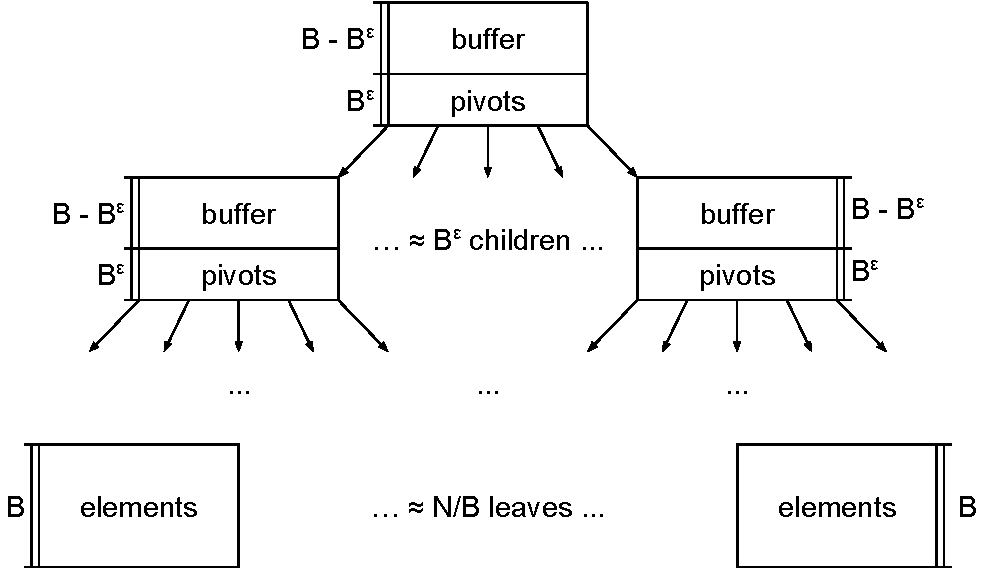
\includegraphics[width=.8\textwidth]{fig/bet}
  \caption{\label{fig:bet} The \bet.}
\end{figure}

\begin{table}[t]
  \centering
  \begin{tabular}{c | c  c  c}
    \hline
    Data Structure & Insert & Point Query & Range Query \\
    \hline
    B-tree & $O(log_{B}{N})$ & $O(log_{B}{N})$ & $O(log_{B}{N} + k/B)$\\
    \hline
    \bet & $O({log_{B}{N}}/{\varepsilon B^{1 - \varepsilon}})$ & $O({log_{B}{N}}/{\varepsilon})$ & $O({log_{B}{N}}/{\varepsilon} + k/B)$\\
    \hline
    \bet ($\varepsilon=0.5$) & $O(log_{B}{N}/{\sqrt{B}})$ & $O(log_{B}{N})$ & $O(log_{B}{N} + k/B)$ \\
    \hline
  \end{tabular}
  \caption{\label{tab:betbtree} The asymptotic IO costs of B-tree and \bet.}
\end{table}

Table~\ref{tab:betbtree} shows the comparison of asymptotic IO costs
between the B-tree and the \bet.
A \bet with node size $B$ partitions each interior node to have
one $(B-B^{\varepsilon})$-size buffer and $B^{\varepsilon}$ pivots.
The resulting tree height is $O(log_{B^{\varepsilon}}{N})=O(log_{B}{N}/\varepsilon)$.
A point query, which follows a root-to-leaf path,
needs to perform $O(log_{B}{N}/\varepsilon)$ IOs.
Similarly, a write is flushed $O(log_{B}{N}/\varepsilon)$ times,
while each flush is done for at least
$O((B-B^{\varepsilon})/B^{\varepsilon})=O(B^{1-\varepsilon})$ writes.
Thus, the amortized cost of each write is $O(log_{B}{N}/(\varepsilon B^{1 - \varepsilon}))$.
If we set $\varepsilon = 0.5$, the \bet has the same asymptotic IO costs for
reads but much better IO costs for writes.

One important change in the \bet is that the IO costs of reads and writes
are asymmetric.
Read-before-write is free in B-trees because a write must go through
the root-to-leaf path anyway, paying the IO cost of fetching all nodes along
the way, and the read-before-write fetches exactly the same set of nodes.
However, in the \bet, most writes can be resolved in the root, so
read-before-write can ruin the performance of the \bet.

To this end, \texttt{upserts} are introduced in the \bet to reduce
read-before-write.
An \texttt{upsert} is a message describing how the old value of the key should
be mutated to become the new value.
Like other writes, new \texttt{upserts} are put to the root.
When an \texttt{upsert} meets the old value during a node flush,
the mutation of this \texttt{upsert} is applied to the old value.
With \texttt{upserts}, reads need to collect \texttt{upsert} messages along
the root-to-leaf path and apply these \texttt{upsert} when the old value is
found, but this doesn't incur additional IOs.
One example is using key/value pairs as counters, the \bet can have
\texttt{upsert} messages describing the amount of increment so that it doesn't
have to read the old value before incrementing.

\subsection{\betrfs}

\begin{figure}
  \centering
  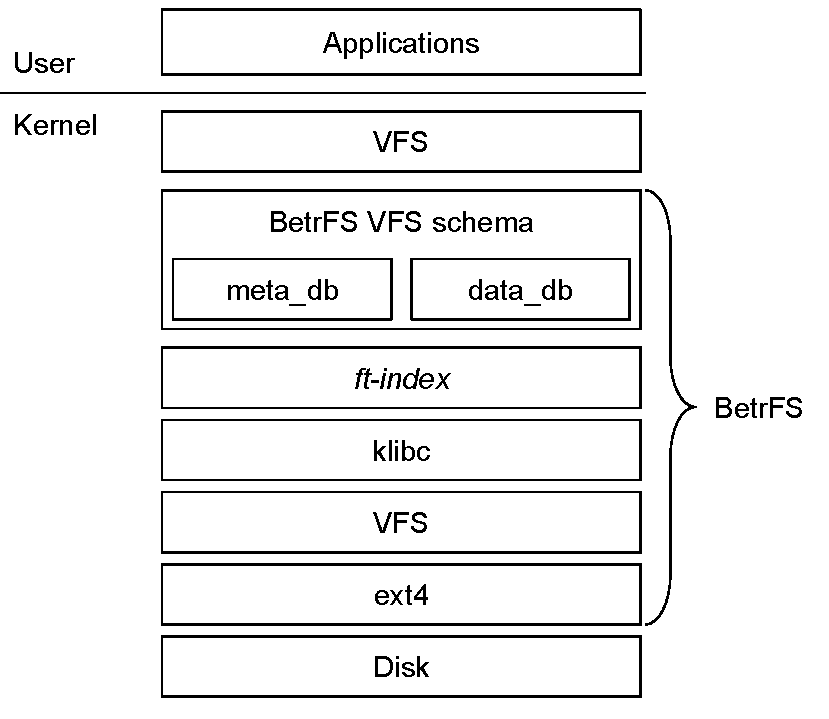
\includegraphics[width=.5\textwidth]{fig/betrfs}
  \caption{\label{fig:betrfs} The \betrfs architecture.}
\end{figure}

\betrfs~\cite{betrfs1,betrfs1tos,betrfs2,betrfs2tos,betrfs3,betrfs4} is a Linux
in-kernel file system built upon \textit{ft-index}~\cite{ftindex},
which implements the \bet and exposes a key-value interface.
The architecture of \betrfs is shown in Figure~\ref{fig:betrfs}.
\betrfs interacts with ft-index through point operations, such as \texttt{put},
\texttt{get} and \texttt{del}, as well as range queries with cursors
(\texttt{c\_getf\_set\_range} and \texttt{c\_getf\_next}).
\betrfs also uses the transaction interface of ft-index to execute multiple
operations atomically.
A redo log and periodic checkpoints (every 5s) in ft-index ensure that changes
can be made persistent on the underlying storage media.

Ft-index cannot be integrated into a Linux kernel module easily because
it is a userspace library that calls \texttt{libc} functions and
\texttt{syscalls}.
We built a shim layer called \texttt{klibc} which implements all functions
ft-index requires.
By implementing those functions in \texttt{klibc} instead of directly modifying
ft-index,
we are able to migrate ft-index into the kernel module intact.

\betrfs uses two key/value indexes to store the metadata and data in a file
system.
One \texttt{meta\_db} maps full-paths to \texttt{struct stat} structures.
Another \texttt{data\_db} maps (full-path + block number) to 4KB blocks.
When the VFS needs the metadata, \betrfs queries the \texttt{meta\_db} with the
full-path and constructs the corresponding inode from the \texttt{struct stat}.
Likewise, when a dirty inode needs to be written, the \texttt{struct stat} is
assembled from the inode and written to the \texttt{meta\_db} with the
full-path key.
Blocks of a file are fetched and written by the full-path and the indexes of
blocks.
Although other block granularity is possible, 4KB is the natural block size
because it is the same as the page size in the Linux page cache.

Full-path indexing is desirable because it offers locality.
With full-path indexing, all keys under one directory are contiguous in the
keyspace.
This, combined with the large node size (4MB) used in \bets, means a large
amount of data are stored close to each other on disk.
After \betrfs fetches one 4KB block of some file from the disk, all nodes along
the root-to-leaf path are present in memory.
Thus, a subsequent fetch to some other block in the same file or another
file under the same directory is likely to be resolved in memory, which
significantly increases performance and IO efficiency.

In \betrfs, in order to avoid read-before-write, writes can proceed without
fetching the old block to memory.
Conventional file systems must read the old block from the disk to the page
cache before writing to that block (a complete overwrite can proceed without
fetching the old block, but it is now implemented in any file system).
However, as described in Section~\ref{subsec:bet}, \bets have asymmetric read
and write costs, so read-before-write should be avoided.
In \betrfs, if the corresponding block is not in memory, an \texttt{upsert}
message describing the offset and the length of this write.
When this message meets the old value during a flush, the change is applied.

\subsection{Making \betrfs better}

\bets and full-path indexing give the first version of \betrfs (\betrfsOne)
good random write performance and good locality.
For example, \betrfsOne is 12.53x faster in creating 3 million small files and
6.86x faster in doing \texttt{find} in the Linux source directory than other
file systems.

However, there are problems with full-path indexing.
Deleting the Linux source directory takes 2.33x longer and renaming the Linux
source directory takes 1.07x longer than other file systems.
We tried to solve these problems in the second version (\betrfsTwo).

\subsubsection{Delete}
In \betrfsOne, each 4KB block is stored as one key/value pair in the \bet.
Deleting a file requires one \texttt{del} call for each block.
This becomes costly when the file is large.

\betrfsTwo introduces a \rd message that deletes a whole range of key/value
pairs.
This is possible because the \bet, unlike the B-tree, is a message-based
data structure.
A \rd, like all other write operations, injects a \rd message of its range into
the root of the \bet.
While the \rd message is flushed down the \bet, it identifies all old messages
in its range and removes them from the \bet.
Thus, when the \rd message reach the leaf, all previous messages in its range
are removed from the \bet.

\subsubsection{Rename}

Rename is a longstanding problem in full-path indexing.
With full-path indexing, all data and metadata are associated with full-path
keys.
Therefore, a rename needs to update all keys in the source.
Also, because all key/value pairs are sorted by their keys, they must be moved
to the destination.

\betrfsOne uses a simple approach that reads all related key/value pairs, puts
them back with new keys and deletes the old key/value pairs.
The cost of this rename increases as the size of the source increases.

\betrfsTwo tries to bound the rename cost at the schema level.
Instead of full-path indexing, \betrfsTwo uses zoning (relative-path indexing).
Zoning divides the directory hierarchy into zones.
Full-path indexing is kept inside a zone while indirection is used between
zones.

\begin{figure}
  \begin{subfigure}{.5\textwidth}
    \centering
    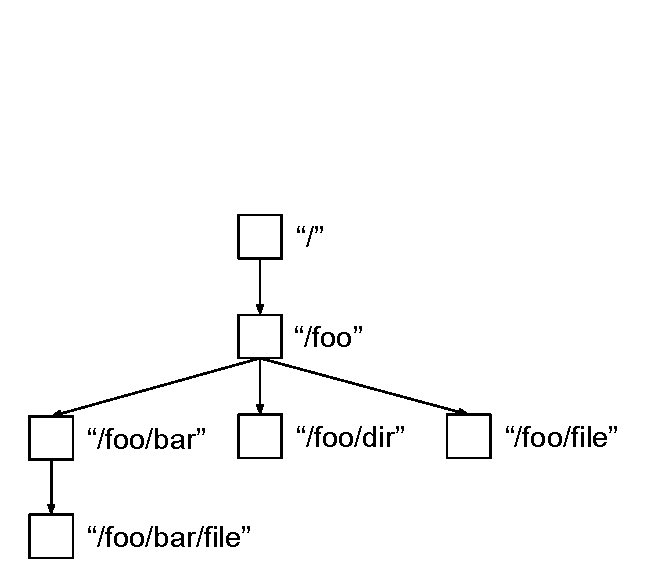
\includegraphics[width=.9\linewidth]{fig/FPI}
    \caption{\label{subfig:FPI} Full-path indexing.}
  \end{subfigure}
  \begin{subfigure}{.5\textwidth}
    \centering
    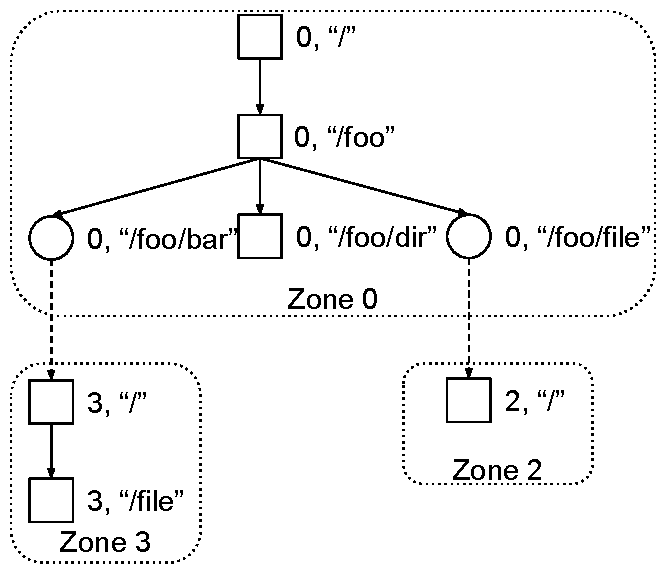
\includegraphics[width=.9\linewidth]{fig/RPI}
    \caption{\label{subfig:RPI} Zoning.}
  \end{subfigure}
  \caption{\label{fig:zoning} Full-path indexing and zoning.}
\end{figure}

For example, in Figure~\ref{subfig:RPI}, directory ``/foo/bar'' forms
its own zone (zone-id 3).
The metadata stored with key (zone-id 0, ``/foo/bar'') (root zone-id is always
0) directs \betrfs to the fetch the metadata of key (zone-id 3, ``/'').
And the file ``/foo/bar/file'' is stored with key (zone-id 3, ``/file'').

Zoning tries to balance locality and rename performance through the target zone
size.
Locality is still maintained within a zone with full-path indexing, so we
want to have bigger zones to pack more things together.
On the other hand, renaming something that is not a zone root still involves
moving all related key/value pairs, so smaller zones mean lower upper-bound
on rename cost.

\betrfsTwo picks a target zone size (128KB by default) and tries to keep each
zone close to that size.
If the size of metadata or data under something that is not a zone root
grows too big, \betrfsTwo does a zone split which moves all related key/value
pairs to a newly formed zone.
Likewise, if the size of a zone becomes too small, \betrfsTwo merges the zone.
